\documentclass[11pt,notes=hide,aspectratio=169,mathserif]{beamer}
% PACKAGES
\usepackage{graphics}  % Support for images/figures
\usepackage{graphicx}  % Includes the \resizebox command
\usepackage{url}	   % Includes \urldef and \url commands
\usepackage{natbib}
\usepackage{bibentry}  % Includes the \nobibliography command
\usepackage{verbatim}  %Supports comments
\usepackage{booktabs} %Supports \toprule, \bottomrule, etc in tables
\usepackage{etoolbox}  %Supports toggle commands
\usepackage{datetime}
\usepackage{bm}	%Supports bold math \bm
\usepackage[latin1]{inputenc}
\usepackage{times}
\usepackage{tikz}
\usepackage{cancel}
\usepackage{graphicx}
\usepackage{subcaption}
\usepackage{pgfplots}
\usepackage[export]{adjustbox}
% PACKAGES (that should already be included by your LyX document settings)
\usepackage{amsfonts}  % Lots of stuff, including \mathbb 
\usepackage{amsmath}   % Standard math package
\usepackage{amsthm}    % Includes the comment functions

% CUSTOM DEFINITIONS
\def\newblock{} %Get beamer to cooperate with BibTeX
\linespread{1.2}

% Define custom colors
\definecolor{myRed}{RGB}{204, 0, 0} % Change RGB values for different shades
\definecolor{lightRed}{RGB}{255, 204, 204} % Lighter shade for backgrounds

% Apply custom colors
\setbeamercolor{structure}{fg=myRed}
\setbeamercolor{palette primary}{bg=myRed,fg=white}
\setbeamercolor{palette secondary}{bg=lightRed,fg=white}
\setbeamercolor{palette tertiary}{bg=myRed,fg=white}
\setbeamercolor{palette quaternary}{bg=lightRed,fg=white}
\setbeamercolor{titlelike}{parent=palette primary}
\setbeamercolor{block title}{bg=myRed,fg=white}
\setbeamercolor{block body}{bg=lightRed,fg=black}


% IDENTIFYING INFORMATION
\title{Politics and Local Provision of Public Goods: Evidence from Chicago}
\author[John Ruf]{John Ruf}
\date{\monthname[\the\month] \the\year}

% THEMATIC OPTIONS
\setbeamercovered{transparent}
\usetheme{Dresden}
\pgfplotsset{compat=1.10}
\usecolortheme{default}
\usefonttheme{professionalfonts}
\beamertemplatenavigationsymbolsempty
\setbeamertemplate{footline}[frame number]{}

% BACKUP SLIDE NUMBERING
\usepackage{appendixnumberbeamer}

%SETTINGS
\newtoggle{shortertalk}
\togglefalse{shortertalk}

\begin{document}

%---------------------------------------------------------------------
\begin{frame}[plain]
\titlepage
\note{
	\begin{itemize}
	\end{itemize}
}
\end{frame}

\section{Introduction}

\begin{frame}{Motivation}
    How do local politicians allocate infrastructure maintenance and other key public goods?
    \begin{itemize}
        \item (Glaeser 2019) find a strong shortage of road maintenance in the country: is it a political economy problem?
        \item If local politicians cannot be trusted to maintain key infrastructure and roads, that has important welfare implications for optimal placement of ``large'' welfare enhancing projects.
        \item How prevalent would clientelism be if we allocated public resources in a more decentralized manner?
        \item What are the costs of giving local politicians unilateral control over infrastructure maintenance? What magnitude would the benefits like ``local knowledge'' and ``accountability'' need to be to justify this?
    \end{itemize}
\end{frame}
    
\begin{frame}{What do aldermen do?}
    \begin{center}
    \begin{quotation}
        ``I remember crossing California going west, every street was resurfaced almost every year. They always had brand new lighting and then east of California, where Ald. Bernie Stone would lose the precincts consistently, I mean the streets were in shambles.'' \\
    \end{quotation}
    \end{center}
    \raggedleft{ -Ald. Carlos Ramirez-Rosa (35th Ward).}
    \begin{itemize}
        \item Aldermen as Mini-Mayor over Ward
        \begin{itemize}
            \item City council defers to Ward Alderman all internal issues
            \item Eg. \ snow plows, garbage cleanup, sign permits, business licenses, liquor-moratoriums, and of course, construction and zoning.
            \item A relatively new power that aldermen were granted in 1995 is the ability to allocate \$1.5M in infrastructure ``menu'' requests 
        \end{itemize}
    \end{itemize}
\end{frame}
    
\begin{frame}{What is the Aldermanic Menu Program?}
        Alderman have the power to allocate \$ 1.5M on a variety of infrastructure projects. They are given a map of 311 complaints for guidance.
    \begin{itemize}
        \item  5 primary categories:
        \begin{itemize}
            \item \textbf{Streets/CDOT:} Alley/Road/Sidewalk Resurfacing, speed bump replacement, sign installation, Curb and Gutter fixes, etc. 
            \item \textbf{Crime Prevention and Lighting:} Camera installation and street lights
            \item \textbf{Arts:} Murals and Neighborhood Arts programs
            \item \textbf{Schools:} Direct grants to CPS, Sports Fields, Gardens, Auditoriums, Playgrounds, etc. 
            \item \textbf{Parks, Trees, and Gardens:} Tree planting, public garden formation, and park cleanup programs. 
        \end{itemize}
    \end{itemize}
\end{frame}

\begin{frame}{2017 OIG Audit}
        The office of the inspector general (OIG) conducted an audit of the menu program in 2017.
        The audit was scathing. 
        They recommended dismantling the program and reallocating the funds to a more traditional central planning model.
        The primary findings of the audit are given below.
    \begin{enumerate}
        \item  Menu, which serves as the City's primary residential infrastructure
        program, underfunds residential infrastructure needs and results in
        significant funding disparities relative to need between wards.
        \item   In the years 2012 through 2015, the City permitted aldermen to designate
        \$15.1 million of Menu funds for projects unrelated to core residential
        infrastructure.
        \item CDOT allowed at least \$825,292 in Menu spending on projects falling outside
        the appropriate ward boundaries and did not enforce project selection
        submission deadlines.
    \end{enumerate}
\end{frame}
\section{Data Description}

\begin{frame}{Data Description}
    \begin{itemize}
        \item Data was collected from about 3600 pages of PDFs from both the OBM website and from FOIA requests.
        \item There were a total of 43,596 projects listed in these PDFs
        \item Each project was scraped, the intersections of all roads were recorded and then located if they exist, and then located using the Census' geocoding API. If the census API failed, then Google Maps' API was used instead.
        \item In total, 83\% of the projects were successfully located using one of the two above methods.
        \item This dataset contains 41,381 precinct-year observations which record the total amount of spending in a given voting precinct in a given year.
    \end{itemize}
\end{frame}

\begin{frame}{PDF Example}
    \begin{figure}[H]
        \centering
        \includegraphics[width=0.6\textwidth]{input/menu_example2.png}
        \caption{Example of a Menu PDF}
        \label{fig:menu_example}
    \end{figure}
\end{frame}

\begin{frame}{Spending is quite concentrated}
    \begin{figure}[H]
        \centering
        % First subfigure
        \begin{subfigure}[b]{0.45\textwidth} % [b] aligns at the bottom
          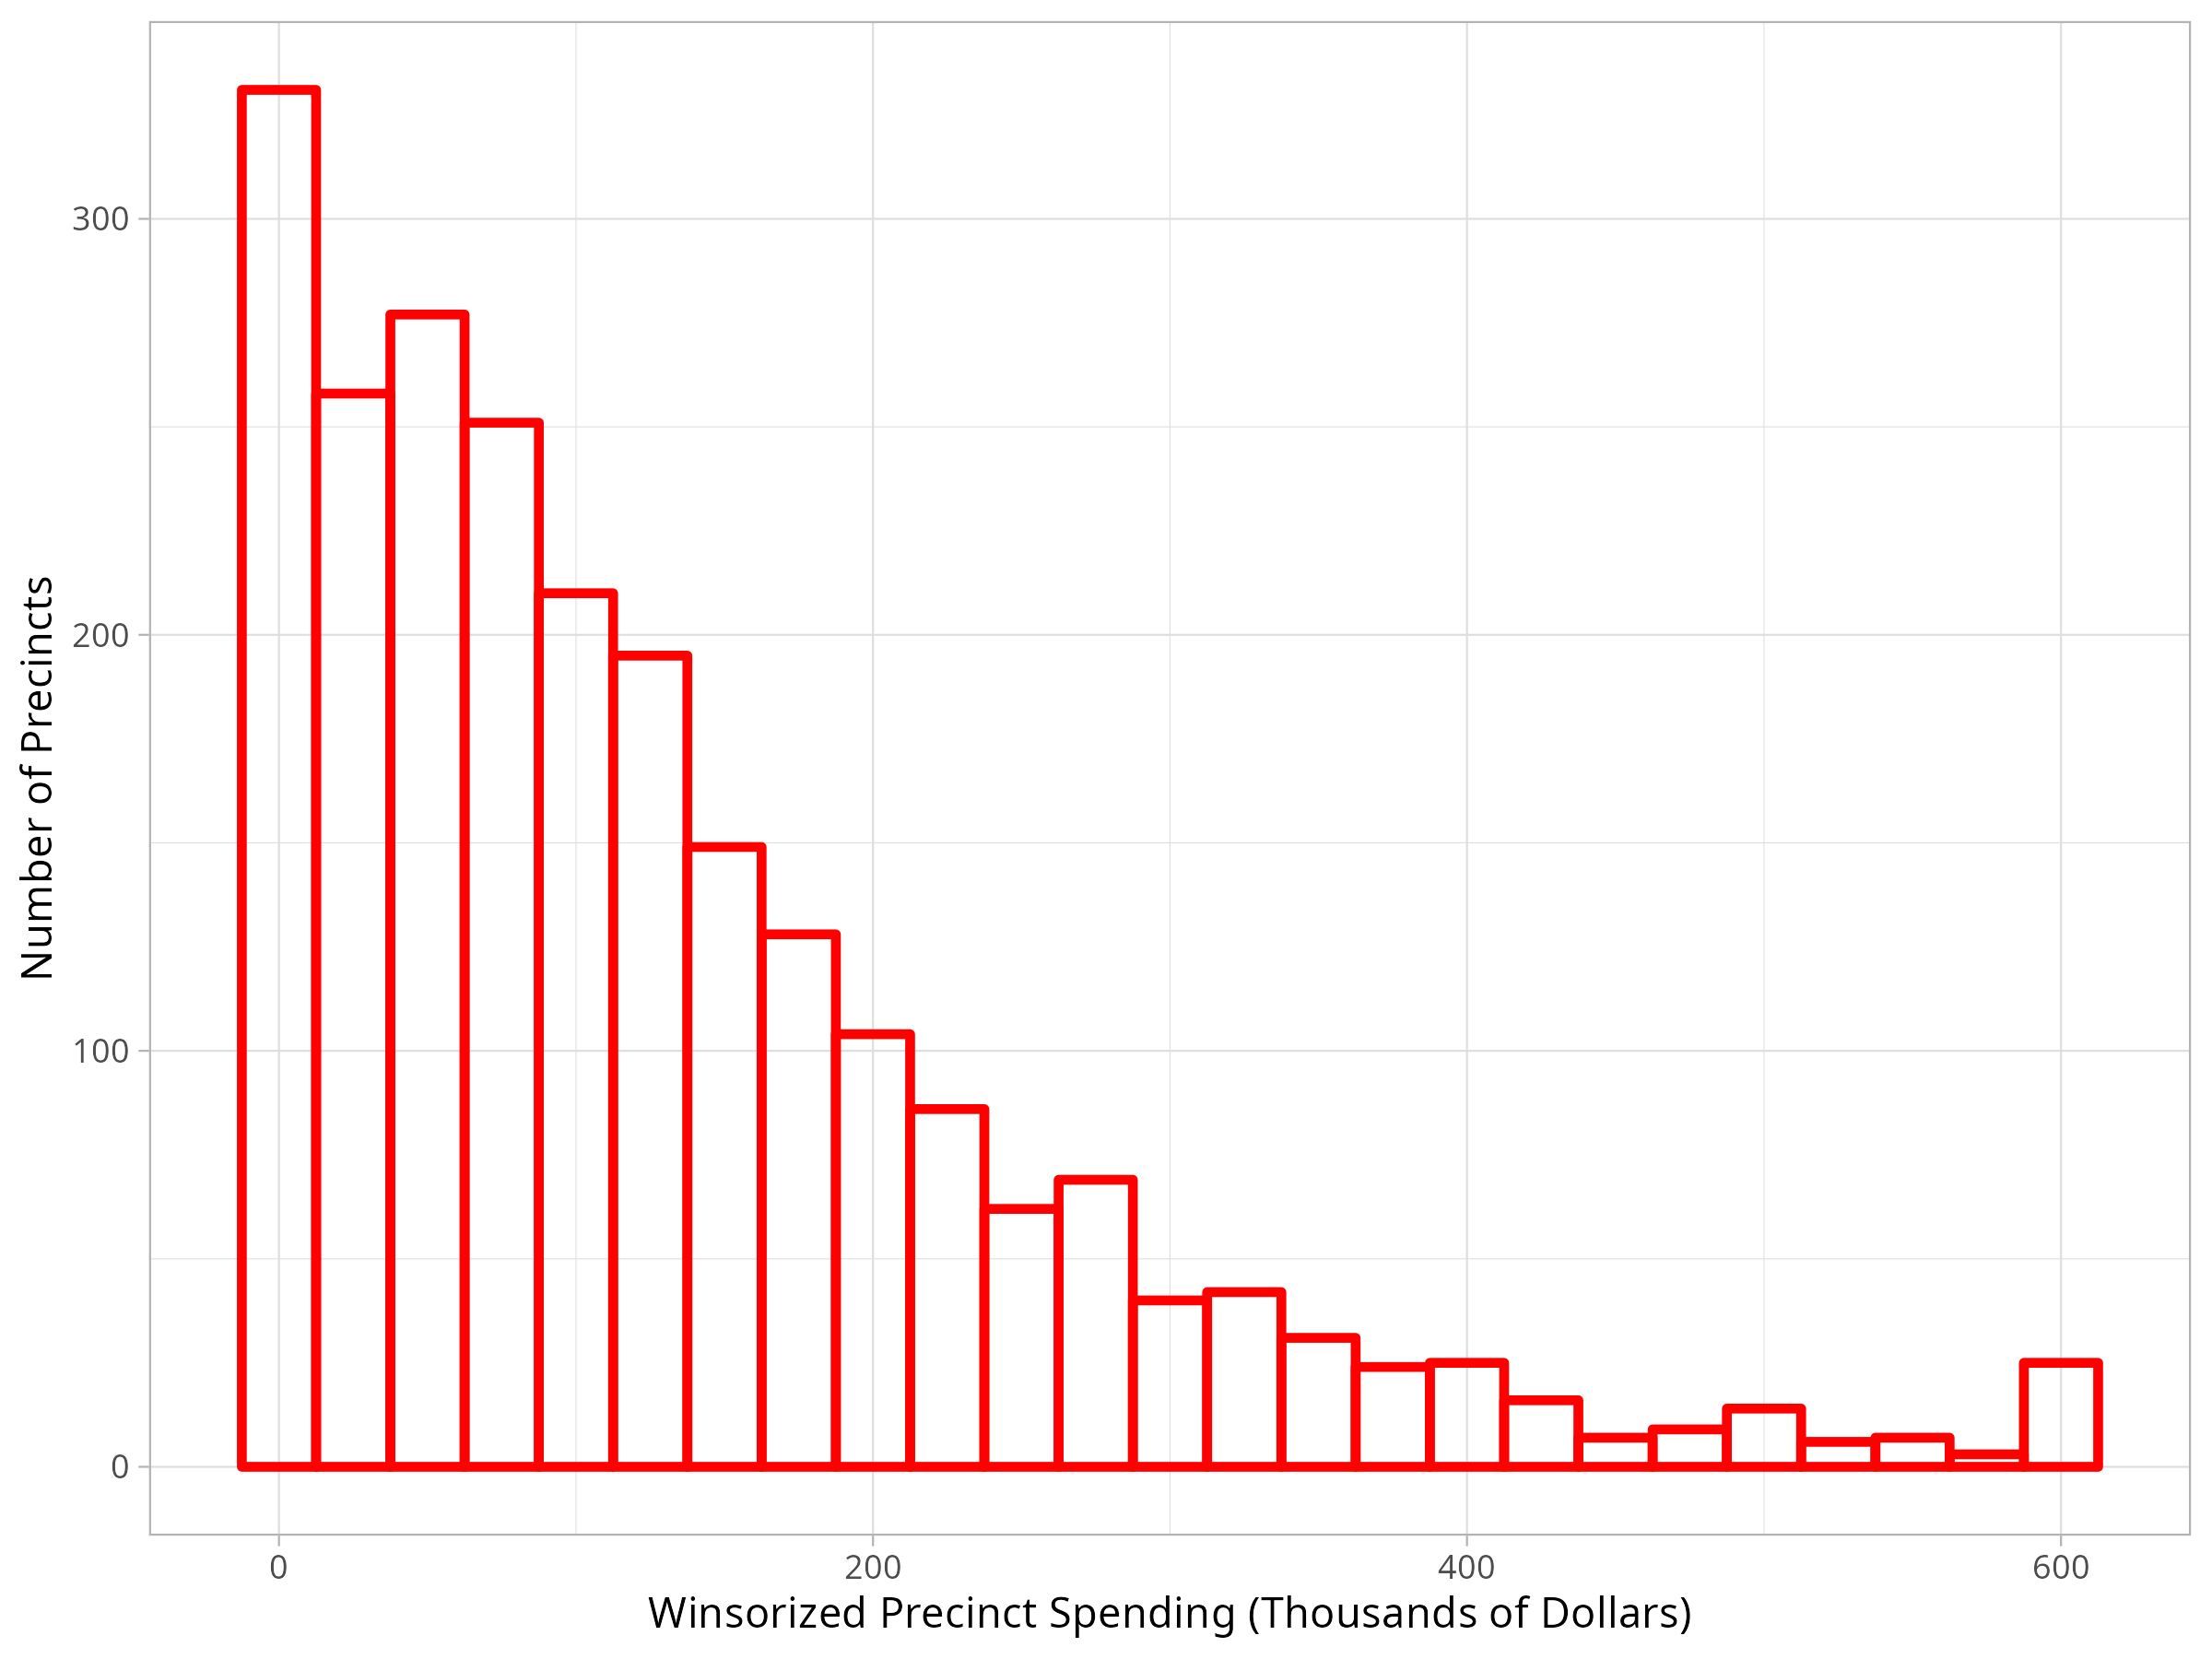
\includegraphics[width=\textwidth]{input/spending_histogram_2005_2011.png}
          \caption{Distribution of Spending per Precinct, 2005-2011}
          \label{fig:sub1}
        \end{subfigure}
        \hfill % This adds some space between the two subfigures
        % Second subfigure
        \begin{subfigure}[b]{0.45\textwidth}
          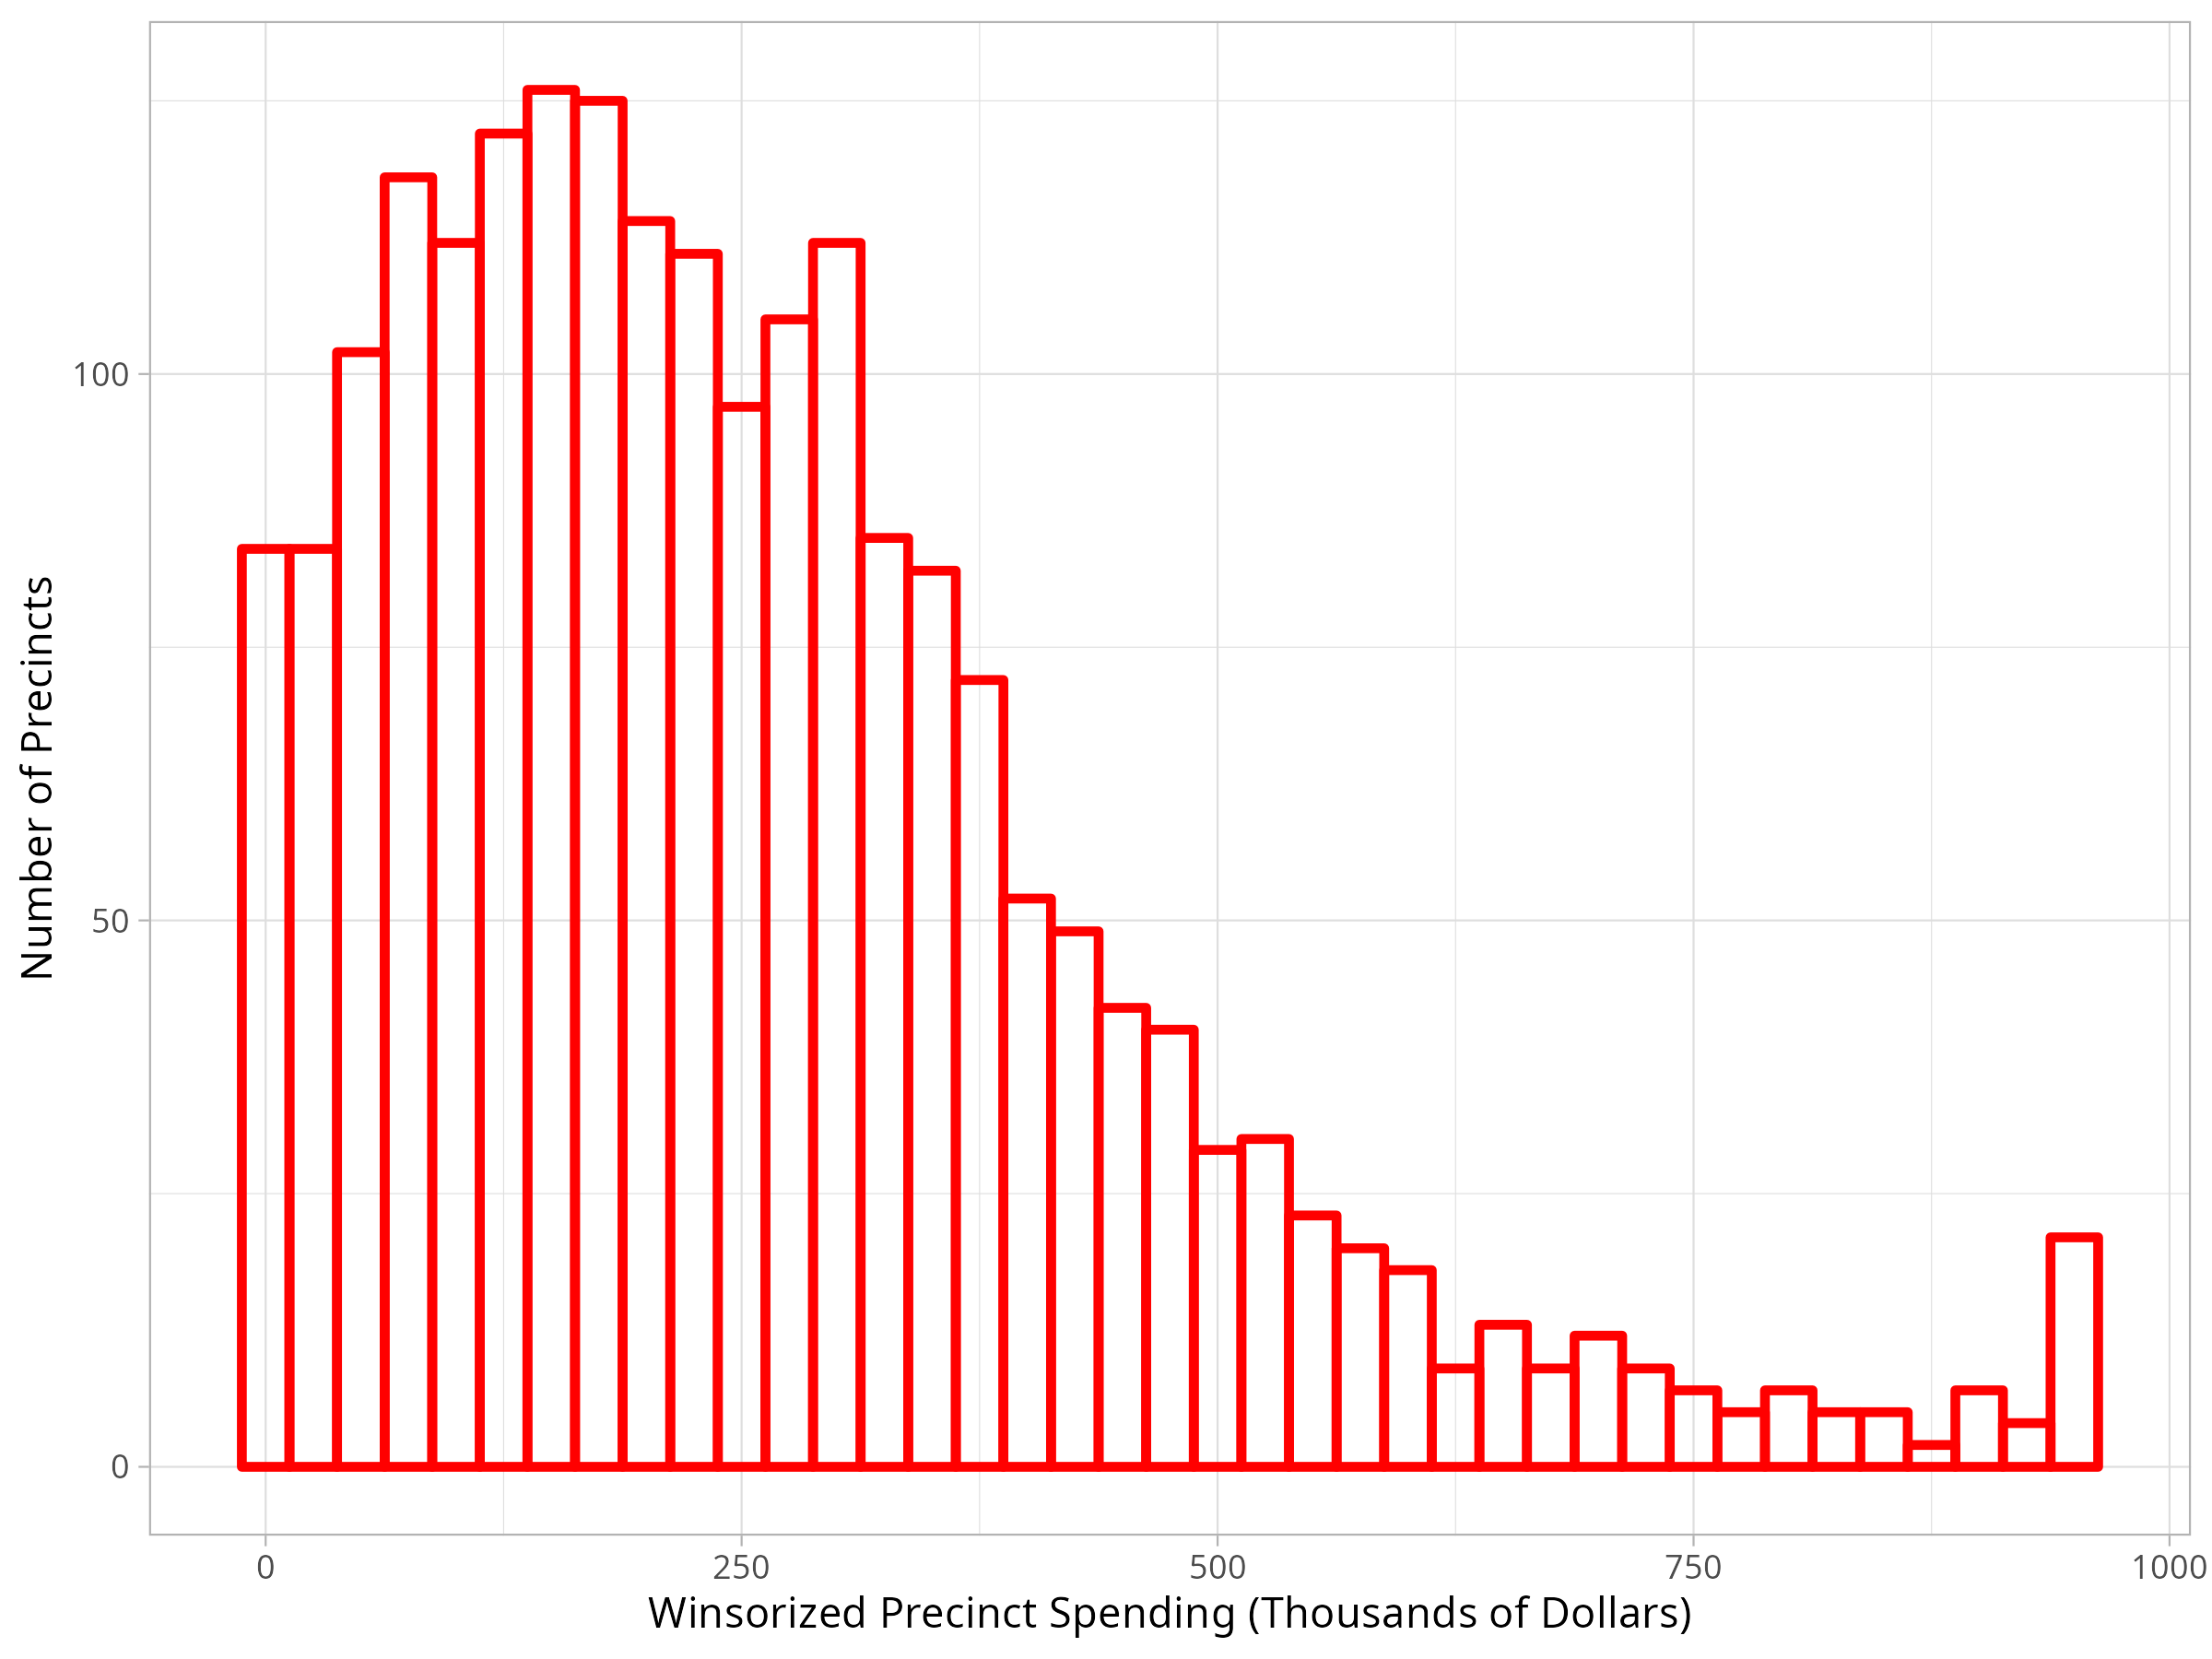
\includegraphics[width=\textwidth]{input/spending_histogram_2012_2022.png}
          \caption{Distribution of Spending per Precinct, 2012-2022}
          \label{fig:sub2}
        \end{subfigure}
      
        \caption{Distribution of Spending per Precinct for both ward maps in the dataset}
        \label{fig:spending_hist}
      \end{figure}
\end{frame}

\begin{frame}{Look at this cool map I made!}
    \begin{figure}[H]
        \centering
        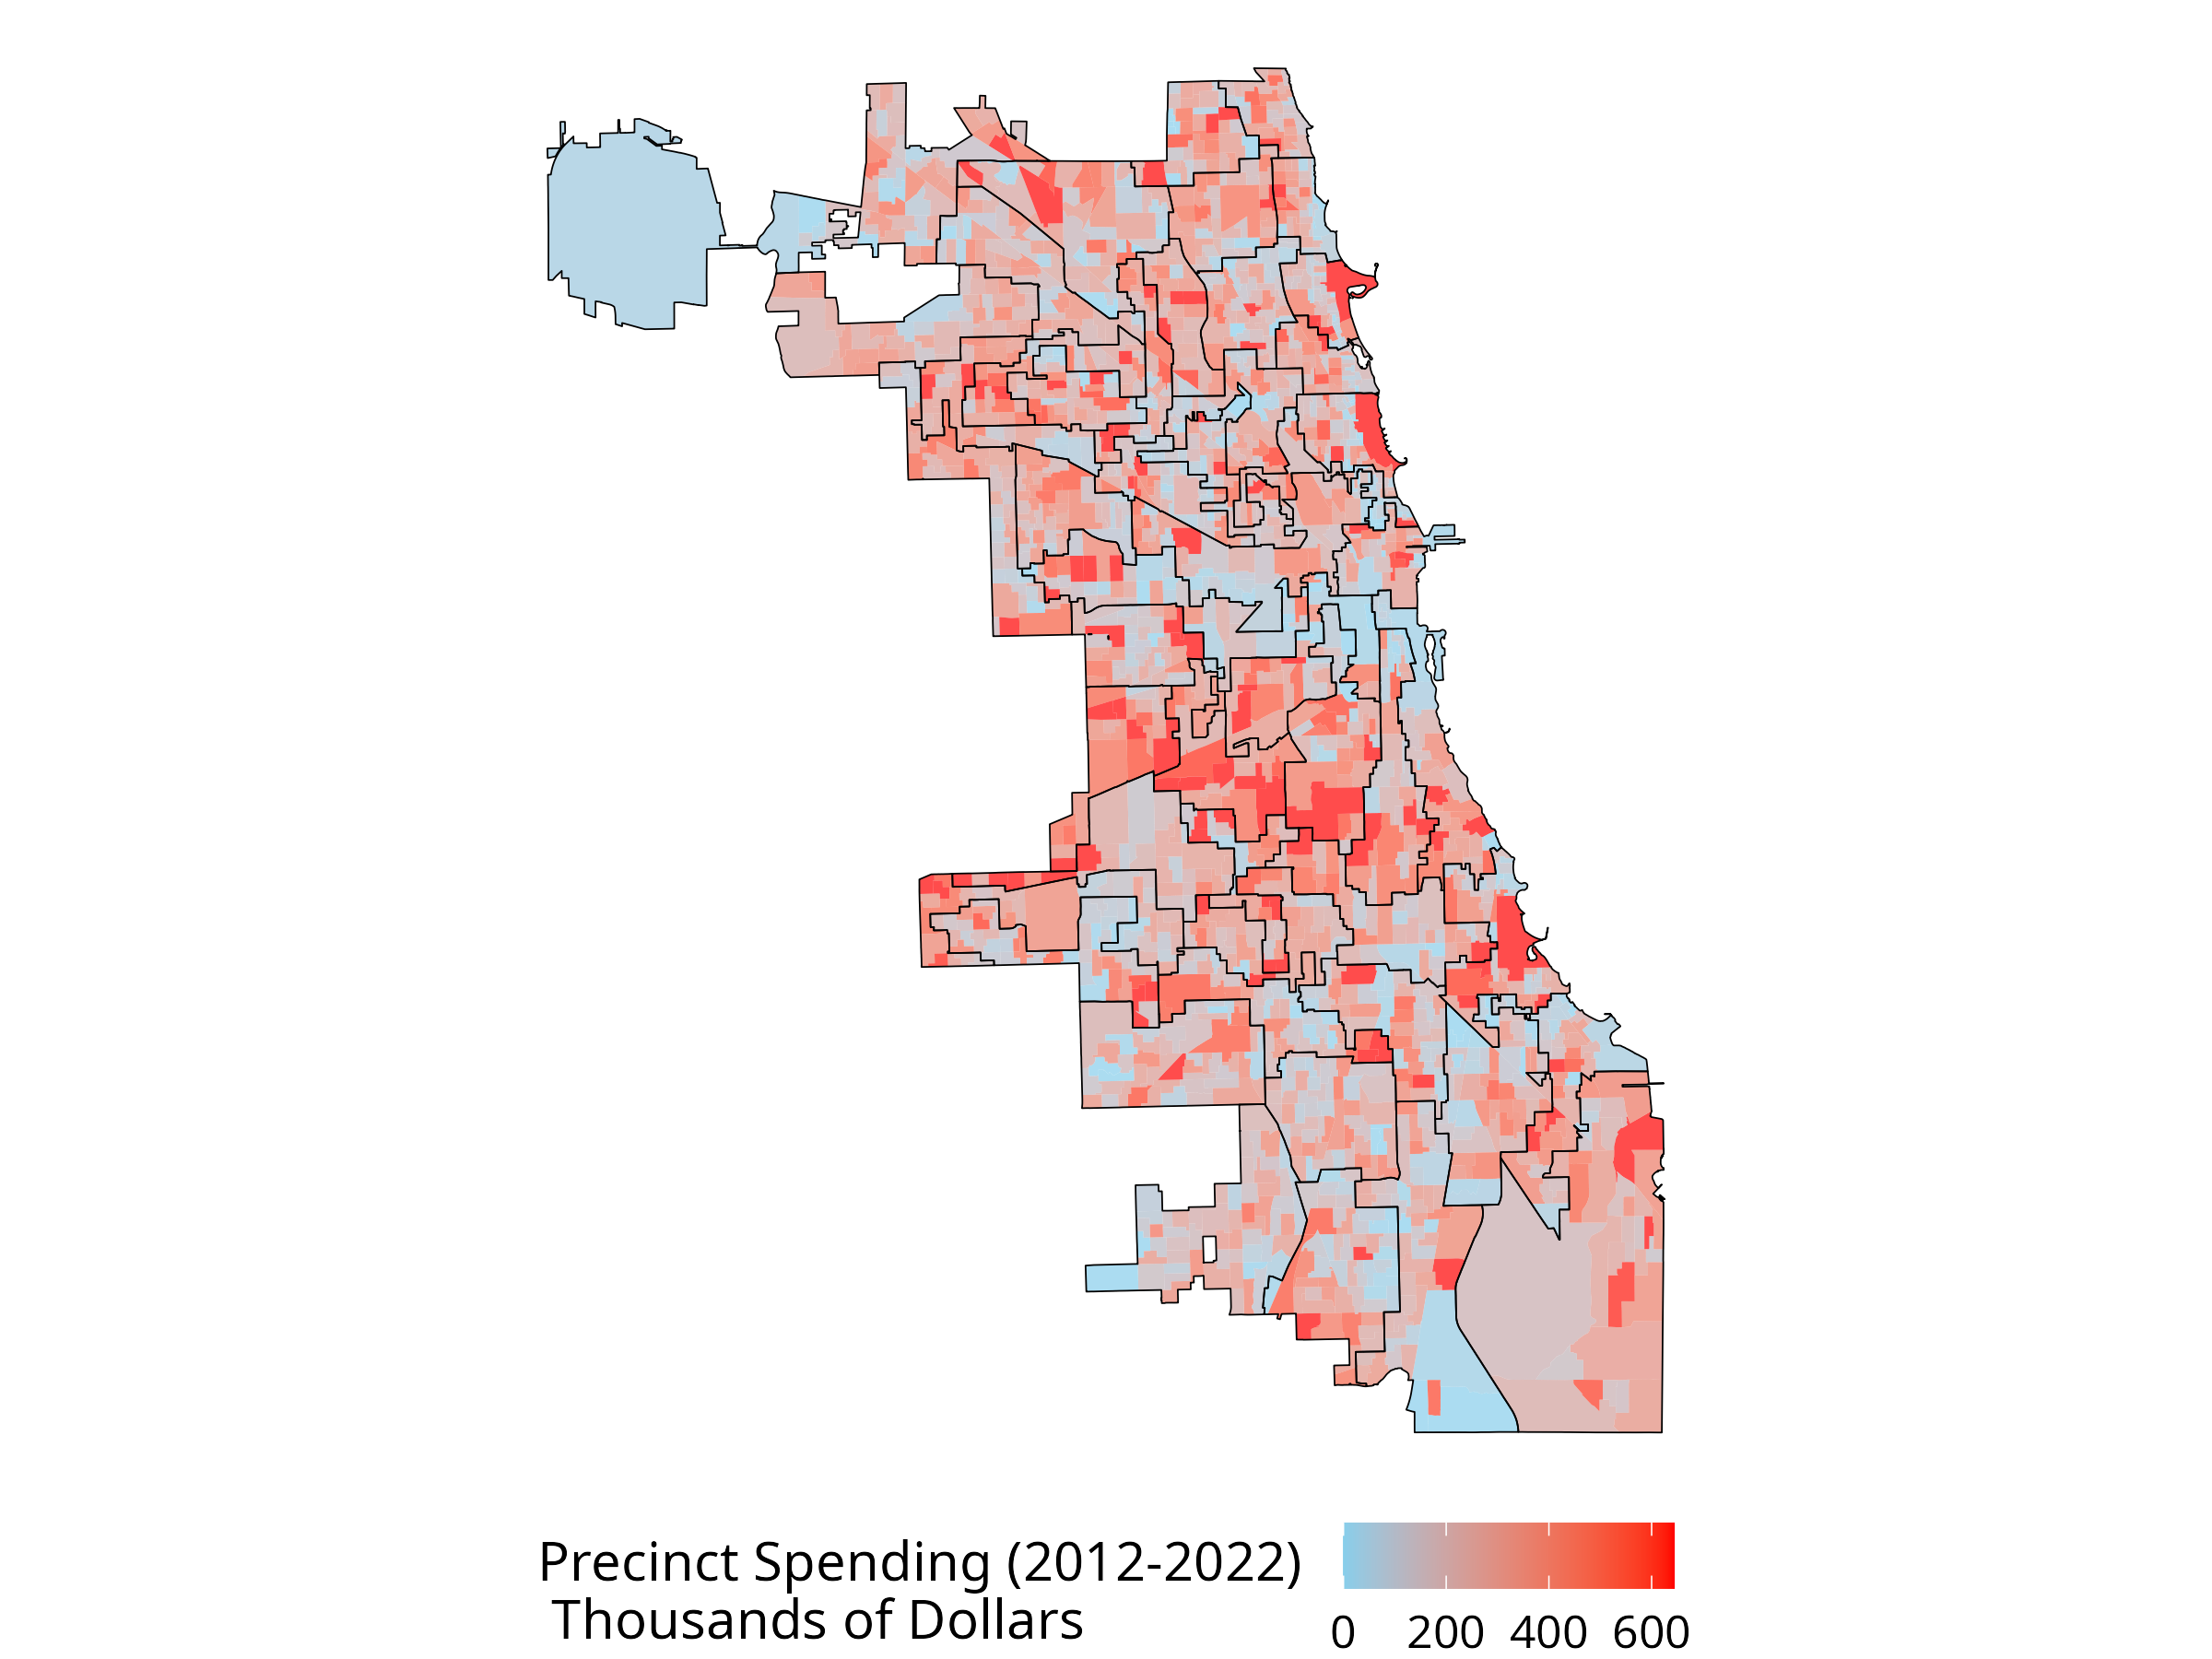
\includegraphics[width=0.6\textwidth]{input/whole_chicago_map_2012_2022.png}
        \caption{Map of Spending per Precinct, 2012-2022}
        \label{fig:spending_map}
    \end{figure}
\end{frame}
\section{Bernie Stone Case Study}
\begin{frame}{Bernie Stone Case Study | Background}
    \begin{itemize}
        \item Bernie Stone was an alderman in Chicago's 50th ward from 1973-2011. 
        \item He was a member of the infamous ``Vrdolyak 29'' -- a group of aldermen who opposed Mayor Harold Washington in the 1980s.
        \item Two of his campaign employees, Anish Eapen and Armando Ramos were charged with vote fraud in 2008
        \item He was well-known in the community for his ``political philosophy'' and Rahm Emanuel described him as ``fiercely loyal to his constituents''
    \end{itemize}
    \begin{quotation}
        ``You take care of the people who take care of you, you know, the people who voted for you, That's not Chicago politics, that's politics 101''
    \end{quotation}
    \raggedleft{ -Alderman Bernie Stone (50th ward)}
\end{frame}

\begin{frame}{Bernie Stone Case Study | Supporting Precincts}
Below are some of the precincts that supported Bernie Stone in the 2007 election and with campaign contributions over the 2005-2011 period.
\begin{figure}[H]
    \centering
    % First subfigure
    \begin{subfigure}[b]{0.3\textwidth} % Adjusted width
    \includegraphics[width=\textwidth]{input/contribution_map_stone_ward_50_2003_2011.png}
    \caption{Campaign contributions to Alderman Stone, 2003-2011}
    \end{subfigure}
    % Second subfigure
    \begin{subfigure}[b]{0.3\textwidth} % Adjusted width
    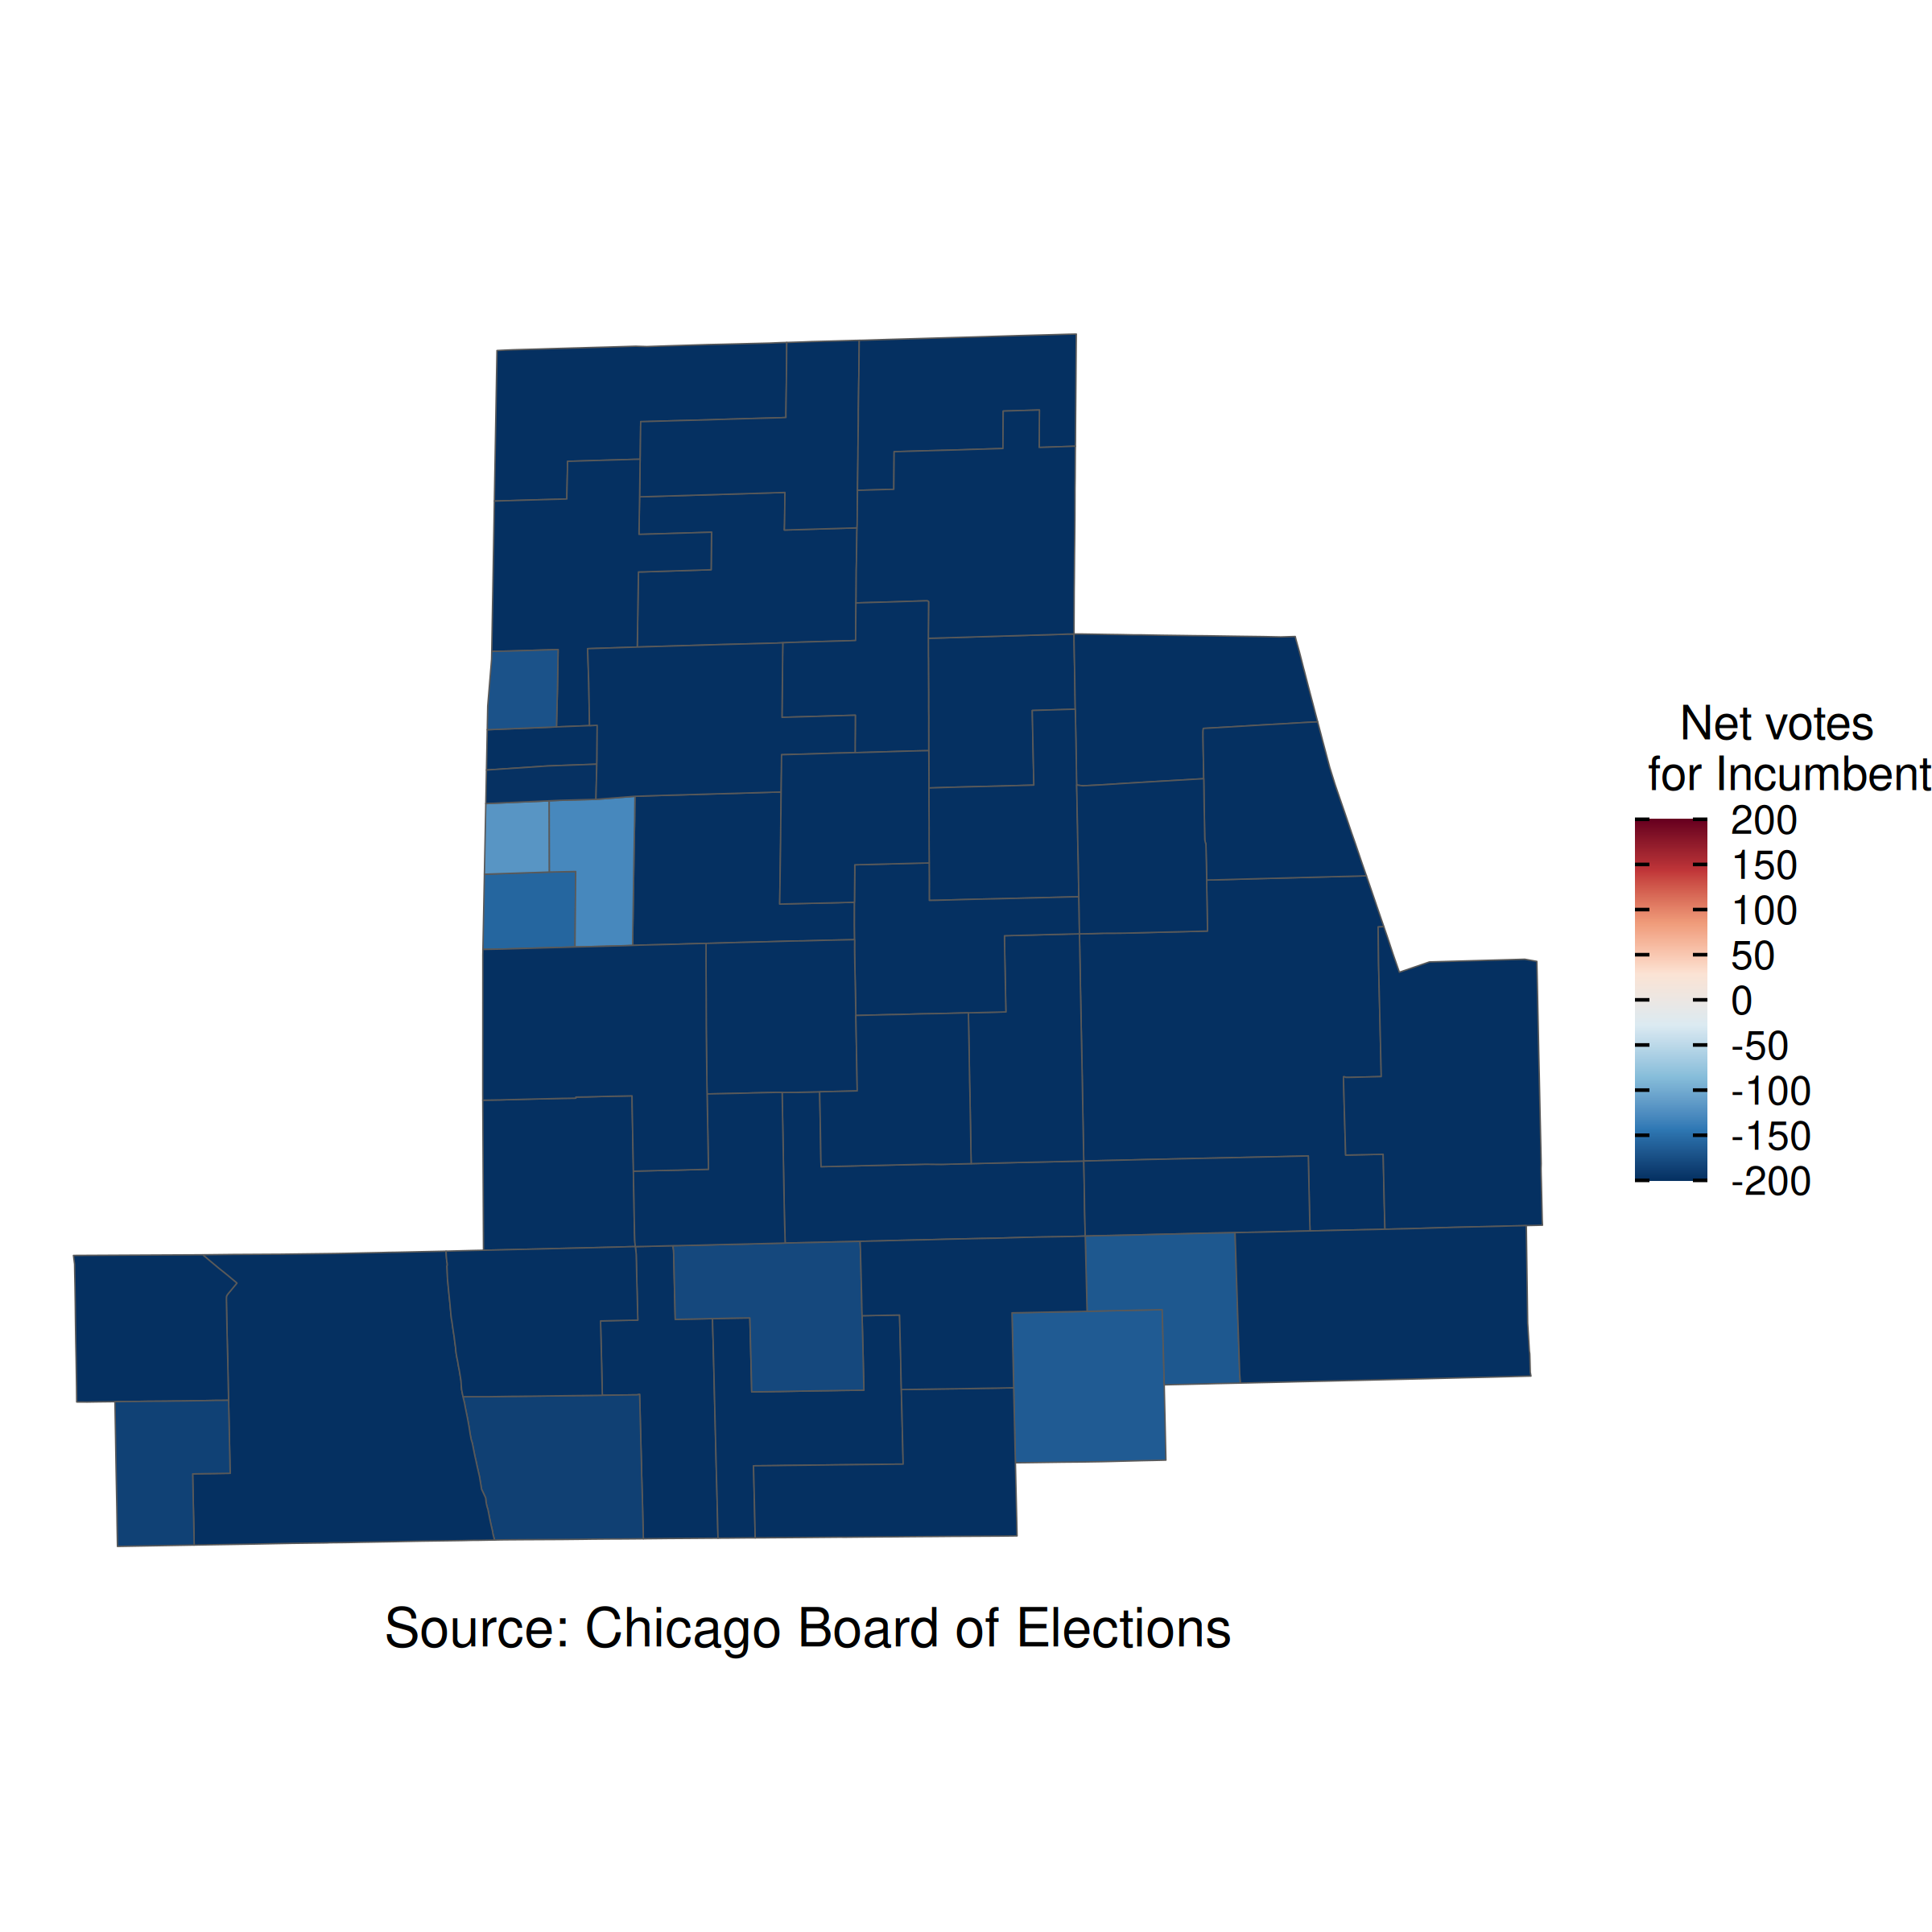
\includegraphics[width=\textwidth]{input/ward_50_2007_runoff_incumbent_precinct_results.png}
    \caption{Net votes for Alderman Stone, 2007}
    \end{subfigure}
    \caption{Distribution of Spending per Precinct for both ward maps in the dataset}
    \label{fig:stone_support_maps}
\end{figure}
\end{frame}

\begin{frame}{Bernie Stone Case Study | Spending Time Series}
Figure\ref*{fig:stone_spending_timeline} shows the average spending per precinct for the top and bottom 8 precincts in the 50th ward by campaign contributions.
This is the first time that this data has been publicly shown.
    \begin{figure}[H]
        \centering
        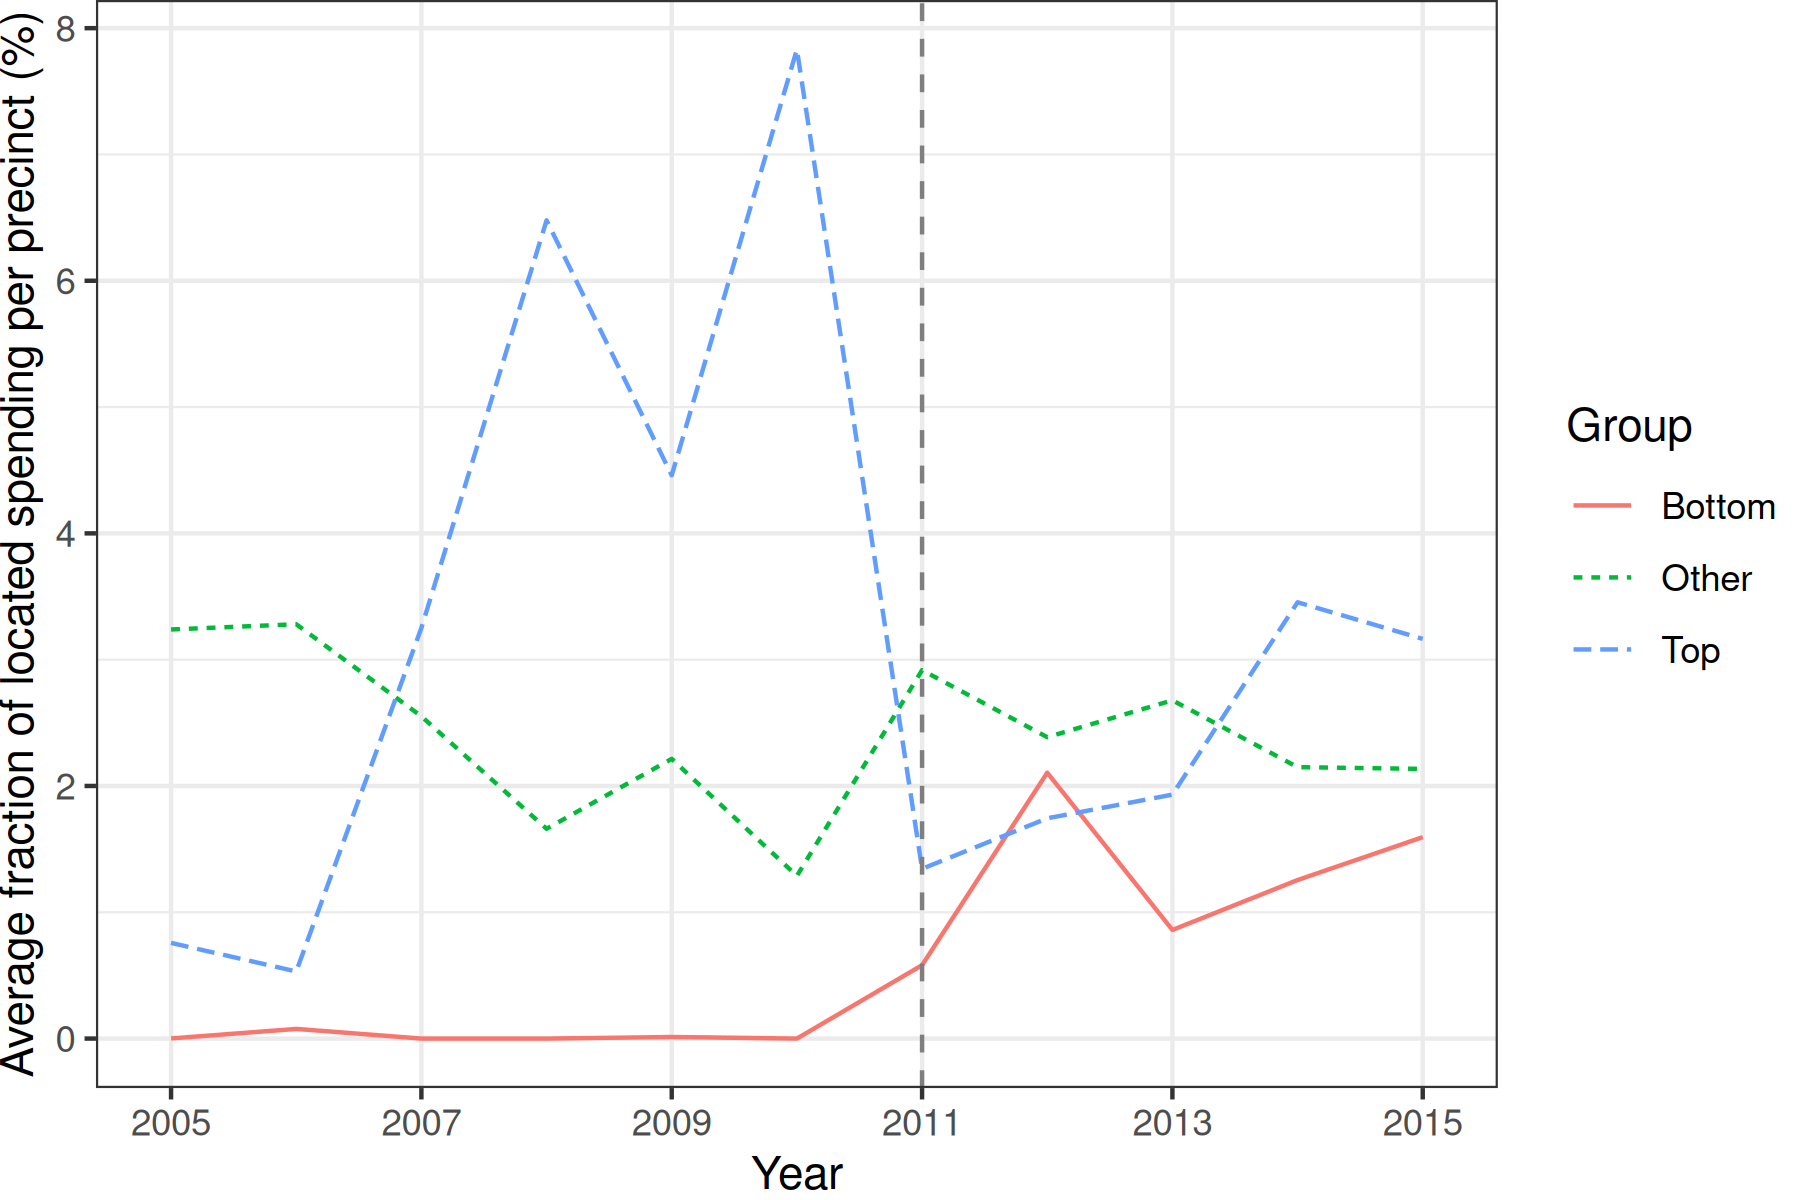
\includegraphics[width=0.4\textwidth]{input/ward_50_contribution_8_precincts_timeline.png}
        \caption{Average Spending per Precinct in the 50th Ward, 2005-2016}
        \label{fig:stone_spending_timeline}
    \end{figure}
\end{frame}

\begin{frame}{Bernie Stone Case Study | Spending Map}
Figure\ref*{fig:stone_menu_maps} compares the chosen distributions of spending before and after Bernie Stone was defeated in 2011.
    \begin{figure}[H]
        \centering
        % First subfigure
        \begin{subfigure}[b]{0.3\textwidth} % [b] aligns at the bottom
        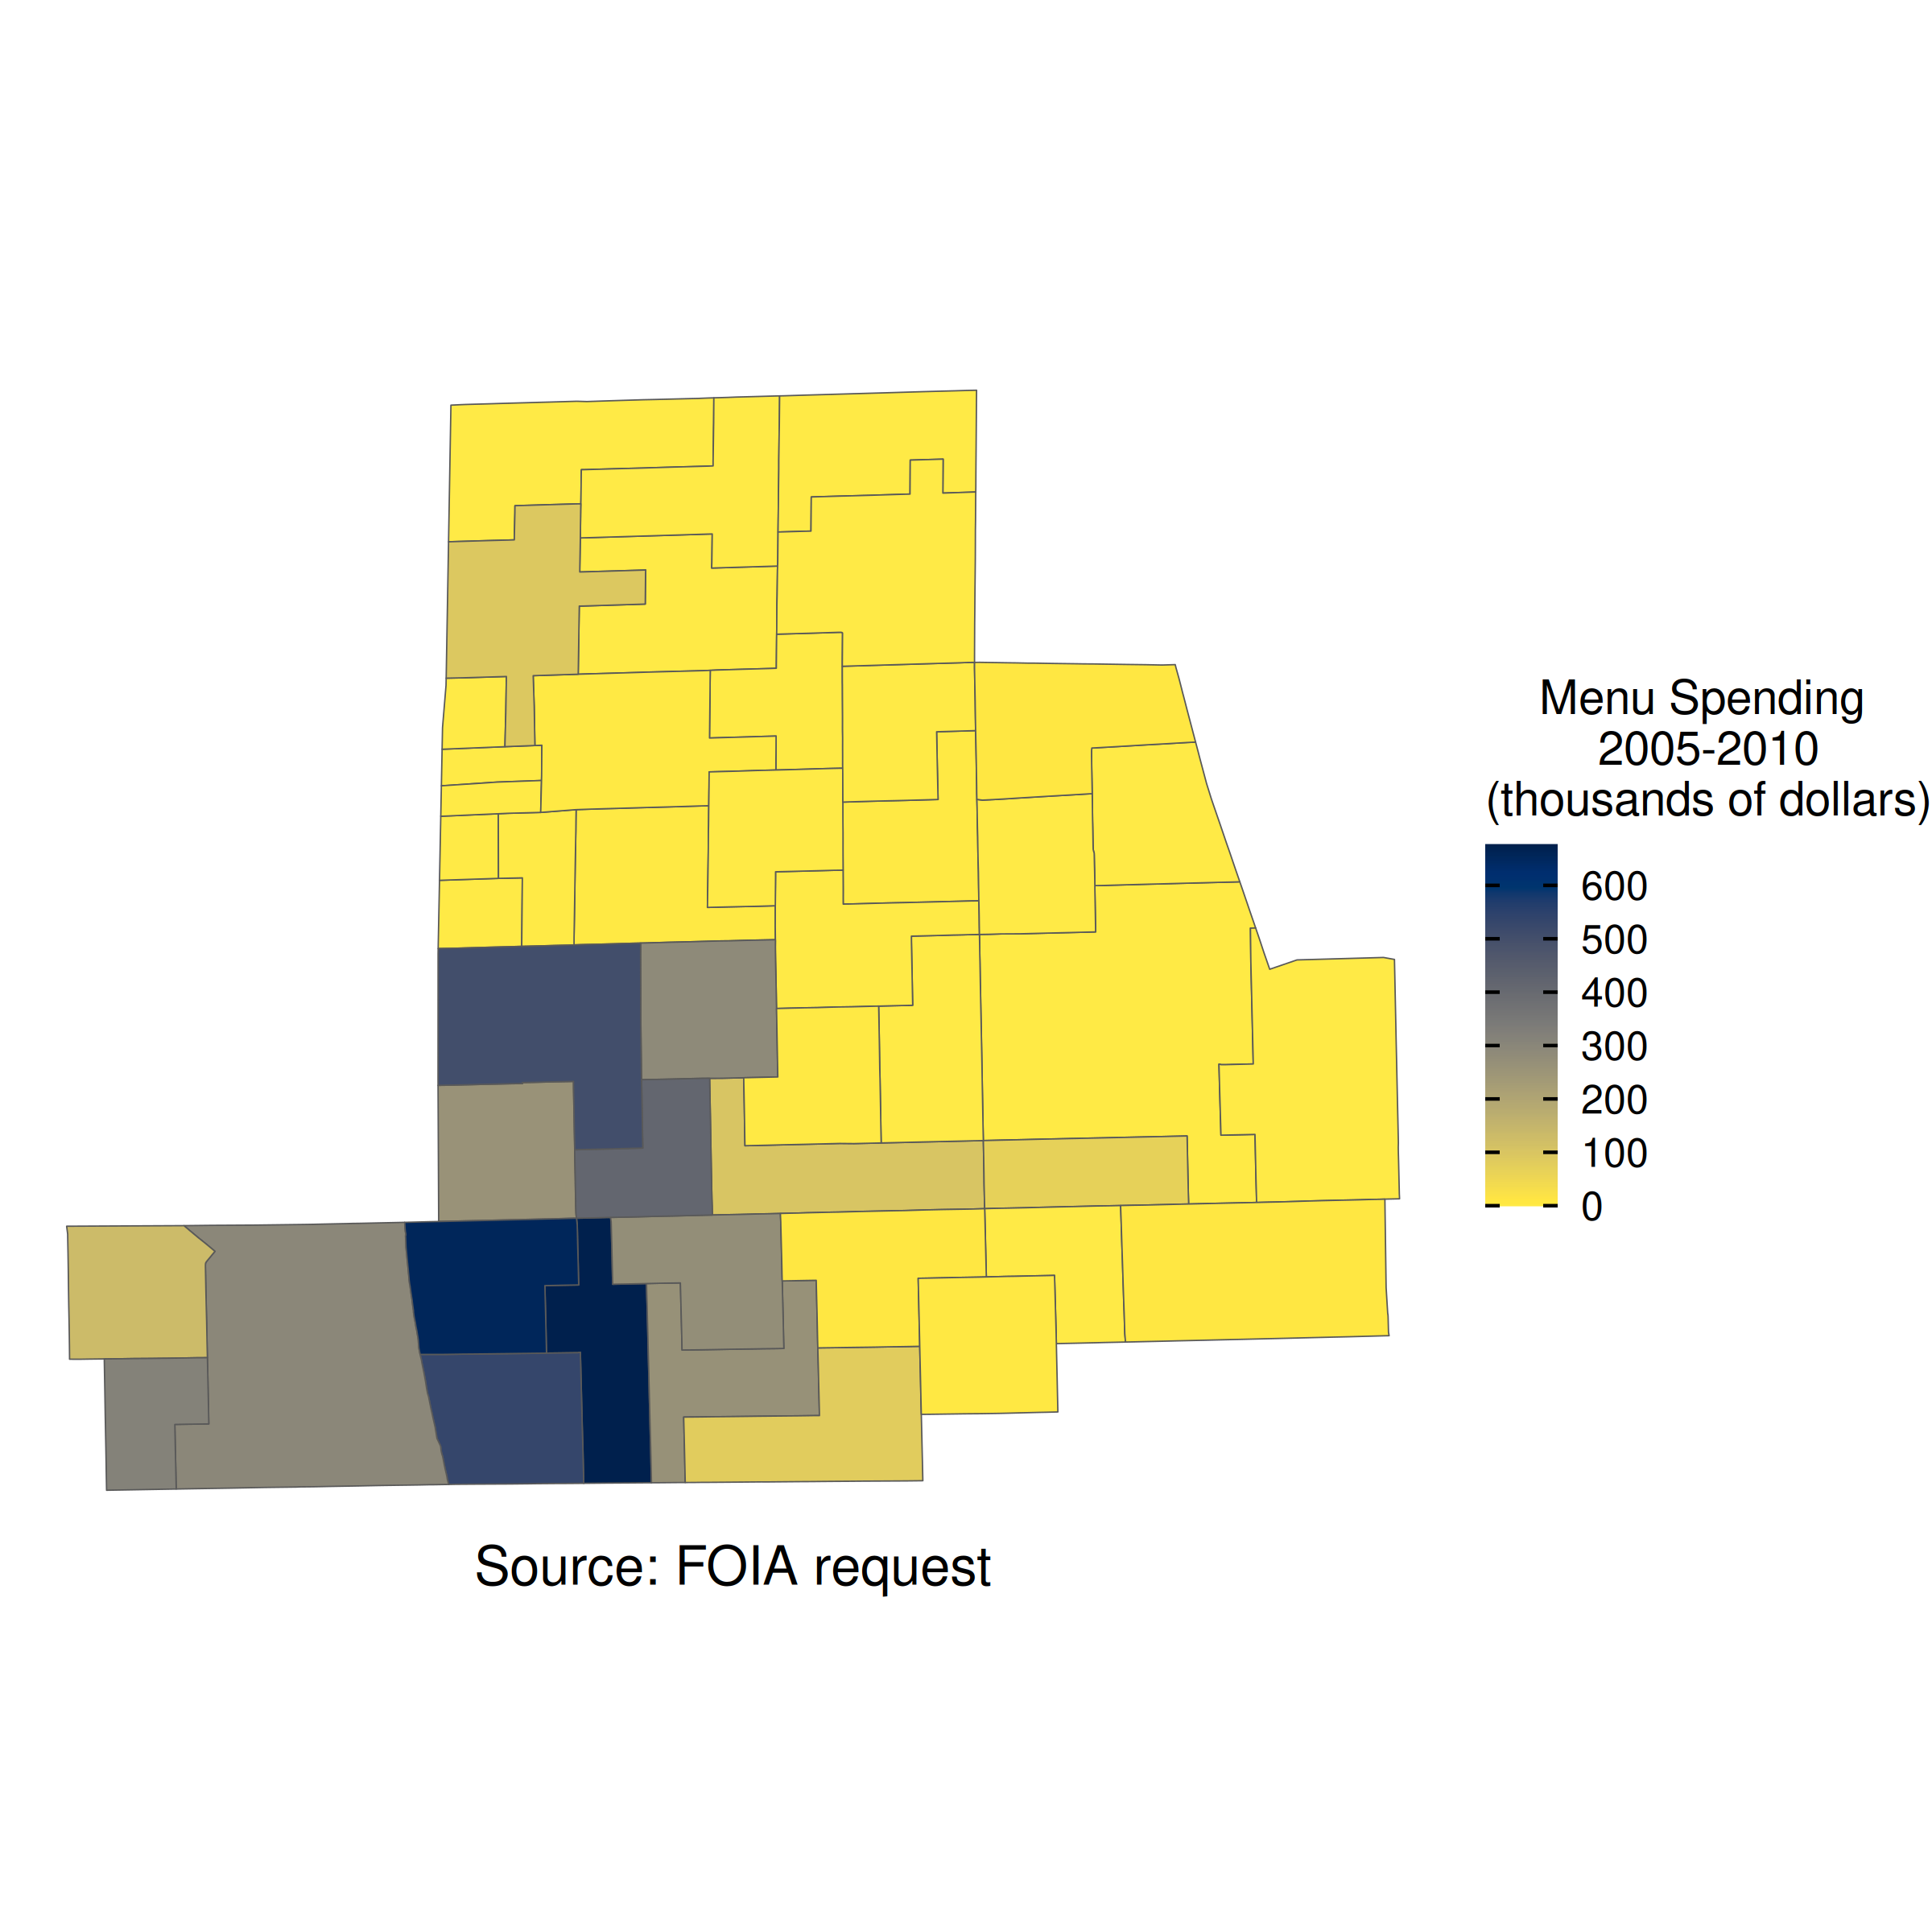
\includegraphics[width=\textwidth]{input/ward_50_menu_map_2005_2010.png}
        \caption{50th Ward Menu Allocation, 2005-2010}
        \end{subfigure}
        % Second subfigure
        \begin{subfigure}[b]{0.3\textwidth}
        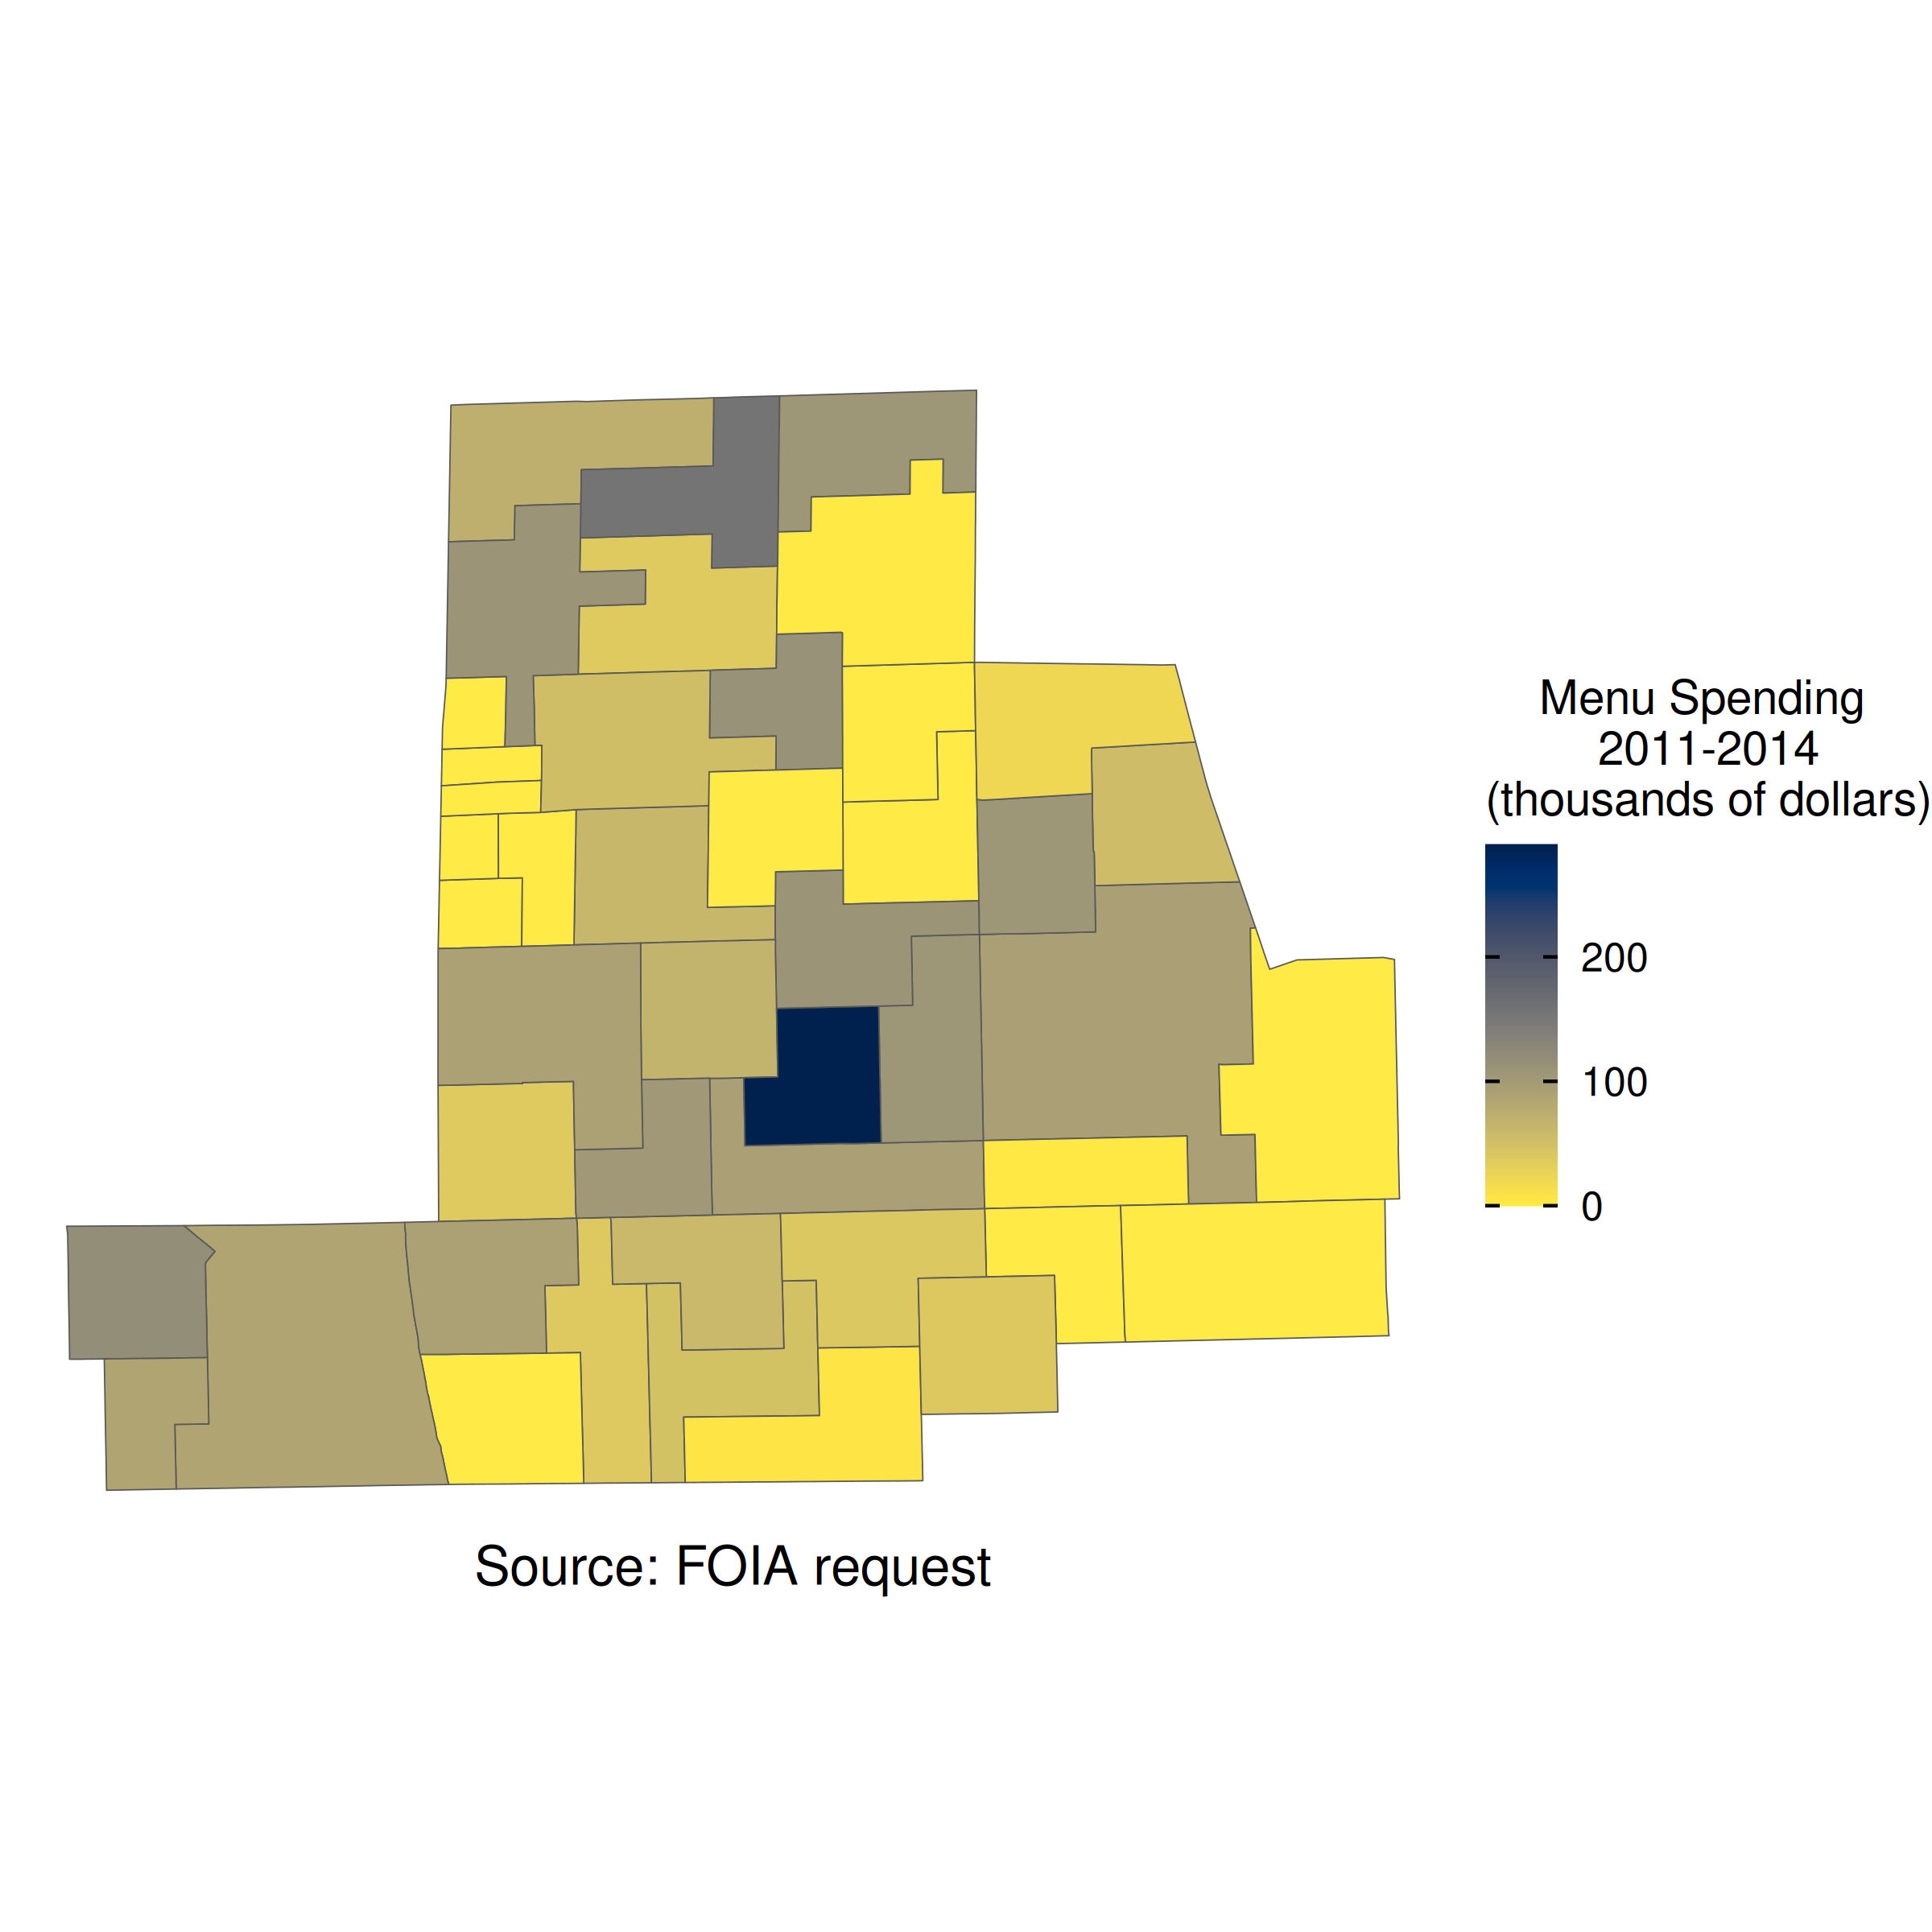
\includegraphics[width=\textwidth]{input/ward_50_menu_map_2011_2014.png}
        \caption{50th Ward Menu Allocation, 2011-2015}
        \end{subfigure}
        \caption{50th Ward Menu Allocation, 2011-2016}
        \label{fig:stone_menu_maps}
    \end{figure}
\end{frame}


\begin{frame}{Resurfacing Data}
    Assuming we want to map a road's characteristics to a predicted value of resurfacing. What resurfacing data might we use?
\begin{itemize}
    \item I have 3881 resurfacing events since 2015
    \item I know the location and blocks of each of these events. 
    \item We observe road closure permits, which are issued by the city to allow for road construction, that gives us timing.
\end{itemize}
\begin{figure}
    \centering
    \includegraphics[width=0.75\textwidth]{input/resurfacing_example.png}
    \caption{Example of Resurfacing Data}
\end{figure}
\end{frame}

\begin{frame}{DiD method}
    \begin{center}
        \begin{tikzpicture}[scale=1]
            \begin{axis}[
                xlabel={$t$},
                ylabel={Flowrate, $V$},
                legend style={at={(1.4,0.5)},anchor=east, text=white, fill=none},
                ymax=10,
                ]
              \addplot[blue, smooth, domain=0:10] {x*(-0.001)+7-0.01*x^2};
              \addplot[red, smooth, domain=0:4.9] {x*(-0.001)+4-0.01*x^2};
              \addplot[red, smooth, domain=5.1:10, unbounded coords=jump] {x*(-0.001)+9-0.01*x^2};
              \draw[dotted] (axis cs:5,0) -- (axis cs:5,8.89);
              \legend{Treated,Control}
            \end{axis}
          \end{tikzpicture}
    \end{center}
\end{frame}

\begin{frame}{Dingel's critique: What if roads don't all decay at the same speed?}
    \begin{center}
        \begin{tikzpicture}[scale=1]
            \begin{axis}[
                xlabel={Time, $t$},
                ylabel={Flowrate, $V$},
                legend style={at={(1.4,0.5)},anchor=east, text=white, fill=none},
                ymax=10,
                ymin=0
                ]
              \addplot[blue, smooth, domain=0:10] {x*(-0.001)+7-0.01*x^2};
              \addplot[red, smooth, domain=0:4.99] {x*(-0.3)+4-0.03*x^2};
              \addplot[red, smooth, domain=5.01:10, unbounded coords=jump] {x*(-0.001)+9-0.005*x^2};
              \draw[dotted] (axis cs:5,0) -- (axis cs:5,8.89);
              \legend{Treated,Control}
            \end{axis}
          \end{tikzpicture}
    \end{center}
\end{frame}

\begin{frame}{Structural Option: Assume that `fresh' roads have identical density-flow mapping}
If DiD is unconvincing, then we can try to find a structural option.

Let $Q_{t,r} (\rho_t, k,r)$ be the density-flow mapping for a road $r$ of type $k$ at time $t$, and let $t^*$ be the time at which the road was resurfaced.
We assume the following:
\begin{align*}
    \forall \ t \ s.t. \ \epsilon+t^* >t \geq t^*: Q_{t,r}(\rho_t, k) = Q_{t^*}(\rho_t)
\end{align*}
Then we can find $\mathbf{E}[Q_{t^*}|\rho_t, k]$, and can compute road-specific treatments ($\gamma_r$):

\begin{align}
    \gamma_{r} =  Q_{t^*}(\rho_{t^*},k)-Q_{t_b,r}(\rho_{t_b}, k) 
\end{align}

Where $t_b$ is the time before resurfacing.

Key problem: We'll only be able to identify treatment effects for roads with densities and types covered by the menu data. 
\end{frame}

\section{Results}

\begin{frame}{Result Table| Close Election Design}
These null results are robust to the choice of number of `top` and bottom precincts included.
    \begin{table}[ht]
        \centering
        \caption{Comparison of Average Treatment Effects: Competitive Election Designs}
        \label{tab:att_comparison_close_election}
        \scalebox{0.85}{% Scale down the table by 15%
        \begin{tabular}{lcc}
        \hline
         & Least Supporting Precincts ATT & Most Supporting Precincts ATT \\
        \hline
        ATT & 0.500 &  -1.511 \\
        Std. Error & 0.451 &  1.120 \\
        95\% Conf. Int. & (-0.384, 1.385) & (-3.705, 0.684) \\
        Pre-Trends P-value & 0.005  & 0.076 \\
        Obs & 1680 & 1680 \\
        \hline
        \end{tabular}
        }% end scalebox
    \end{table}
\end{frame}

\begin{frame}{Results Least Supporting Figure | Close Election Design}
    \begin{figure}[ht]
        \centering
        \includegraphics[width=0.6\textwidth]{input/hte_figure_combined_support_bottom.png}
        \caption{Average treatment effect over time for least supporting precincts: competitive election design}
        \label{fig:att_comparison_close_election_bottom}
    \end{figure}
\end{frame}

\begin{frame}{Results Most Supporting Figure | Close Election Design}
    \begin{figure}[ht]
        \centering
        \includegraphics[width=0.6\textwidth]{input/hte_figure_combined_support_top.png}
        \caption{Average treatment effect over time for most supporting precincts: competitive election design}
        \label{fig:att_comparison_close_election_bottom}
    \end{figure}
\end{frame}


\begin{frame}{Results Table | Indictment Design}
The coefficients are similar in magnitude even when you vary the number of precincts included in the analysis.
Statistical significance fluctuates somewhat.
    \begin{table}[H]
        \centering
        \caption{Comparison of Average Treatment Effects: Indictment Designs}
        \label{tab:att_comparison_corruption}
        \scalebox{0.85}{% Scale down the table by 15%
        \begin{tabular}{lcc}
        \hline
         & Least Supporting Precincts ATT & Most Supporting Precincts ATT \\
        \hline
        ATT & 2.5881 & -1.147 \\
        Std. Error & 0.7776 & 0.3191 \\
        95\% Conf. Int. & (1.064, 4.112) & (-1.772, -0.521) \\
        Pre-Trends P-value & 0.199 & 0.174 \\
        Obs & 1144 & 1144 \\
        \hline
        \end{tabular}
        }% end scalebox
    \end{table}
\end{frame}

\begin{frame}{Results Least Supporting Figure | Indictment Design}
    \begin{figure}[ht]
        \centering
        \includegraphics[width=0.6\textwidth]{input/hte_figure_corruption_bottom_8_precincts.png}
        \caption{Average treatment effect over time for least supporting precincts: indictment design}
        \label{fig:att_comparison_close_election_bottom}
    \end{figure}
\end{frame}

\begin{frame}{Results Most Supporting Figure | Indictment Design}
    \begin{figure}[ht]
        \centering
        \includegraphics[width=0.6\textwidth]{input/hte_figure_corruption_top_8_precincts.png}
        \caption{Average treatment effect over time for most supporting precincts: indictment design}
        \label{fig:att_comparison_close_election_bottom}
    \end{figure}
\end{frame}

\begin{frame}{Conclusions}
    \begin{enumerate}
        \item This collects a brand new policy-relevant dataset and brings it to the public for the first time
        \item Using this data, we verify a long-standing rumor of selective spending in Chicago's 50th ward
        \item A diff-in-diff design shows that selective spending is not happening in competitive elections
        \item Another diff-in-diff design, albeit flawed, shows selective spending is happening at least with aldermen who were indicted for other reasons.
        \item Tidbit: Chi-hack night is using my data to create an app to help citizens track menu spending in their wards.
    \end{enumerate}
    \end{frame}

%---------------------------------------------------------------------
\begin{frame}[plain]
\begin{center}{\LARGE Thank you}\end{center}
\end{frame}

\begin{frame}[plain]
Feel free to come up and ask questions
\begin{center}
	Main Takeaways
\end{center}
\begin{enumerate}
	\item This collects a brand new policy-relevant dataset and brings it to the public for the first time
	\item Using this data, we verify a long-standing rumor of selective spending in Chicago's 50th ward
	\item A diff-in-diff design shows that selective spending is not happening in competitive elections
	\item Another diff-in-diff design, albeit flawed, shows selective spending is happening at least with aldermen who were indicted for other reasons.
	\item Tidbit: Chi-hack night is using my data to create an app to help citizens track menu spending in their wards.
\end{enumerate}

\end{frame}

\begin{frame}{Some other ideas}
	\begin{enumerate}
		\item Steal Olivia Bordeu's JMP border specification and use it to estimate the effect of ward density on the distribution of public goods.
		\item Idea is use precincts to estimate the following equation, where distance is defined by the distance to the nearest border of the ward.
		\item ``central'' precincts should get a disproportionate amount of spending relative to ``border'' precincts
		\item Dense wards (IE: Wards who need less money) should be more willing to spend on border precincts
	\end{enumerate}
		\begin{equation}
			J_i = \zeta \mathbb{1}(\text{Dist}_p >0) + \upsilon \text{Dist}_p + \nu \mathbb{1}(\text{Dist}_p > 0) \times \text{Dist}_p + f_p +\epsilon_{ip}
		\end{equation}
	\end{frame}
%---------------------------------------------------------------------


%\beginbackup
%\appendix
%\input{sections/appendix.tex}

%\bibliographystyle{../bib/aeanobold}
%\nobibliography{../bib/bib.bib}
%\backupend


\end{document}